\chapter{Proposta}


Seguir padrão em desenvolvimento de software é uma premissa básica, pois ao trabalhar com variações dentro de uma organização, a tendência é gerar confusão. Assim, o objetivo deste trabalho é formular um módulo padrão de permissões de acesso, de modo que o mesmo possa ser utilizado por diferentes plataformas, como desktop, web e mobile, eliminando assim este módulo do desenvolvimento de um software e utilizando o trabalho proposto como um Saas provedor das permissões do software cliente a ser desenvolvido.


É bastante comum encontrar frameworks de desenvolvimento de software que automaticamente geram um esquema de configuração de módulos com os perfis de acesso. Entretanto, apesar de ser um facilitador, tal política pode se tornar confusa em algus cenários, a exemplo de uma empresa que trabalha com sistemas sob encomenda, onde o cliente pode até mesmo determinar a linguagem ou framework de desenvolvimento. Nesse caso, a empresa teria que treinar os seus colaboradores a configurar os softwares para cada uma das ferramentas utilizadas, podendo gerar uma confusão.


Diante da possibilidade de manter a configuração dos sistemas de uma mesma instituição com diferentes módulos de permissão, seria ideal que todos os softwares utilizassem um mesmo módulo de configuração de persmissão de acesso, para que esta parte comum, presente na maioria dos softwares, fosse padronizada.


\section{Arquitetura da aplicação}


A aplicação desenvolvida neste trabalho foi arquitetada com o modelo SPA(Single page application) utilizando o AngularJs. Tal arquitetura se tornou tão popular quanto o famoso MVC (Model-View-Controller), e é bastante usada em aplicações web e mobile. SPA basicamente significa codificar menos no server-side e mais no client-side. Assim, boa parte da aplicação passa a ser processada no cliente (dentro do navegador Web).


Vantagens da SPA:
\begin{itemize}

\item Balanceamento da responsabilidade da execução entre cliente e servidor.
\item Menos código do servidor, e mais responsabilidade no cliente;
\item Melhorar a experiência ao usuário (UX) criando interface com usabilidade moderna e de fácil entendimento do usuário;
\item Menor consumo de banda, pois as cargas de dados são feitas por demanda e por AJAX.

\end{itemize}
O grande ator de app SPA é o código Javascript executado no cliente. Toda a aplicação pode ser construída simplesmente manipulando o DOM – Document Object Model de forma nativa, ou com o uso de bibliotecas e frameworks Javascript que auxiliam na construção da aplicação. Estas bibliotecas e frameworks fornecem recursos para manipulação dinâmica do DOM, definição de templates de tela, chamadas assincronas ao servidor, organização do código Javascript, etc. Dentres as diversas bibliotecas Javascript disponíveis no momento, as mais difundidas na comunidade de progamadores estão: AngularJs, VueJs, Backbone, ReactJs, Ember e outras.


No lado servidor, temos a execução das linguagens tradicionais como PHP(Adotada nesse projeto), ASP.NET, JSP, etc, trabalhando também de forma tradicional, servindo arquivos, acessando a banco de dados, tratando as regras de negócios que não podem estar no código JS por questões de segurança. E é neste lado (servidor) que podemos utilizar a arquitetura REST – Representational State Transfer para fornecer serviços do servidor para nossa aplicação SPA. É comum encontrar aplicação SPA utilizando serviços RESTFul. Uma aplicação no servidor que utiliza a arquitetura REST para servir serviços, então é chamada de RESTFul. Neste trabalho, foi desenvolvida uma aplicação RESTFul com o Framework PHP Laravel.


Ao construir uma aplicação utilizando a arquitetura REST, o protocolo HTTP é usado em sua essência, utilizando os métodos de requisição ao servidor: GET, POST, PUT e DELETE (os mais comuns), e cada um deles indica uma determinada ação a ser executada em um recurso específico do servidor.


\begin{figure}
	\label{fig:spa}
	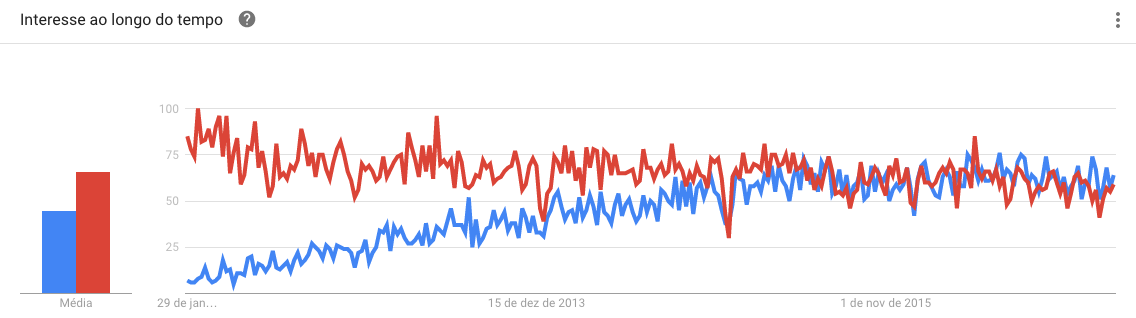
\includegraphics[width=1\textwidth]{img/spa-mvc}
	\caption{Gráfico do Google Trends exibindo comparação entre as pesquisas por SPA e MVC}
\end{figure}


\subsection{Tecnologias utilizadas}


\subsubsection{Laravel framework}


Laravel é um framework PHP livre e open-source para o desenvolvimento de sistemas web que utilizam o padrão MVC (model, view controller). O Laravel foi desenvolvido sob o MIT License, com o código-fonte hospedado no GitHub. Em Agosto de 2015, o Laravel já era o principal framework de projetos PHP no GitHub. 


Algumas características proeminentes do Laravel são sua sintaxe simples e concisa, um sistema modular com gerenciador de dependencias dedicado, várias formas de acesso a banco de dados relacionais e vários utilitários indispensáveis no auxílio ao desenvolvimento e manutenção de sistemas.   


\subsubsection{AngularJs}


AngularJS é um framework JavaScript open-source, mantido pelo Google, que auxilia na execução de single-page applications. Seu objetivo é aumentar aplicativos que podem ser acessados por um navegador web e foi construído sob o padrão model-view-view-model (MVVM).


A biblioteca lê o HTML que contém tags especiais do framework e então executa a diretiva na qual esta tag pertence, e faz a ligação entre a apresentação e seu modelo, representado por variáveis JavaScript comuns. O framework adapta e estende o HTML tradicional para uma melhor experiência com conteúdo dinâmico, com a ligação direta e bidirecional dos dados (two-way data-binding) que permite sincronização automática de models e views. Como resultado, AngularJS abstrai a manipulação do DOM e melhora os testes.


\subsubsection{Bootstrap}


Bootstrap é um popular framework front-end que facilita a criação de sites com tecnologia responsiva.
O Bootstrap possui diversos componentes (plugins) em JavaScript (jQuery) que auxiliam o desenvolvedor a implementar, menu-dropdown, modal, carousel, slideshow, entre outros com facilidade, apenas acrescentando algumas configurações no código.


\subsection{Diagramas UML}


\begin{figure}
	\label{fig:Diagrama de caso de uso}
	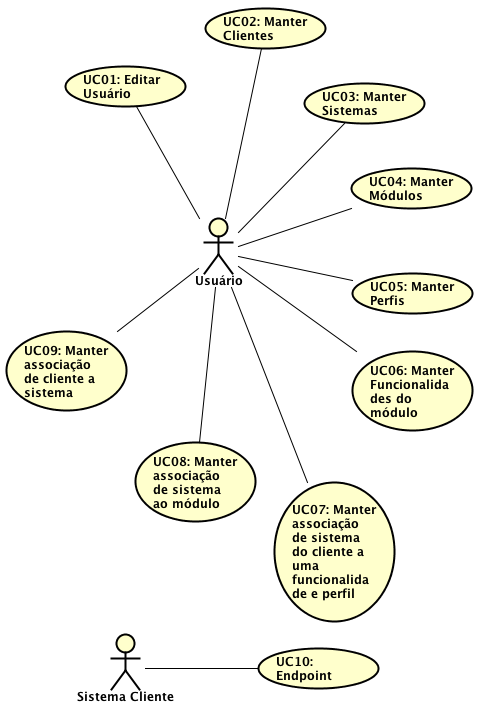
\includegraphics[width=1\textwidth]{img/Diagrama_de_caso_de_uso}
	\caption{Diagrama de caso de uso}
\end{figure}


\begin{figure}
	\label{fig:DER}
	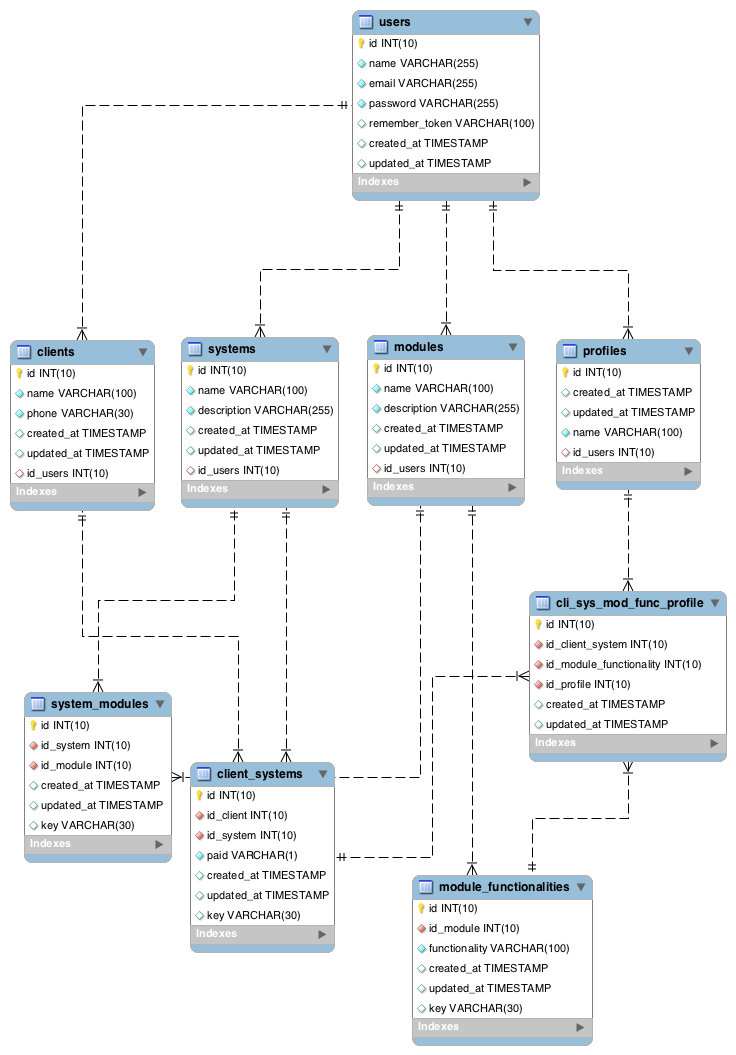
\includegraphics[width=1\textwidth]{img/DER}
	\caption{Diagrama entidade relacionamento}
\end{figure}


%FALTA INSERIR O DIAGRAMA DE CLASSE


\subsection{Funcionalidades}


A fim de apresentar as funcionalidades do sistema proposto, nesta seção serão apresentados os requisitos de acordo com a engenharia de software.


\subsubsection{Requisitos não funcionais}



\begin{itemize}
	
	
\item RN01: Usuários Simultâneos


Descrição: O sistema deverá suportar processamento multiusuário, ou seja, vários usuários poderão utilizar o sistema simultaneamente. 


\item RN02: Segurança 


Descrição: O sistema só permitirá acesso aos dados com autorização. Os usuários deverão se identificar usando um login e uma senha, e a referida senha será criptografada no banco de dados.


\item RN03: Alta disponibilidade 


Descrição: O sistema deverá ter disponibilidade de aproximadamente 99 porcento do tempo. 


\item RN04: Desempenho


Descrição: Os tempos de resposta das consultas não devem ultrapassar 3 segundos.


\end{itemize}
	

\subsubsection{Requisitos funcionais}


\begin{itemize}
	
	
\item RF 01: Login


Descrição: O sistema deve conter tela de login com os campos email e senha. Após inserção dos dados, o sistema deve validar os dados e caso positivo, encaminhar o usuário ao sistema. Caso os dados sejam inválidos, exibir mensagem de erro para o usuário.


\item RF 02: Edição de usuário


Descrição: O sistema deve conter um formulário que seja carregado com os dados do usuário da sessão e permitir a atualização dos dados. Este caso de uso está relacionado ao UC01.


\item RF 03: Cadastro de cliente


Descrição: O sistema deve conter um formulário para cadastro de clientes. Após a inserção de um registro, o sistema deve automaticamente exibir o registro em formato de edição e conter botão para ir a uma consulta que liste os clientes cadastrados para o usuário da sessão. Este caso de uso está relacionado ao UC02.


\item RF 04: Cadastro de sistema


Descrição: O sistema deve conter um formulário para cadastro de sistemas. Após a inserção de um registro, o sistema deve automaticamente exibir o registro em formato de edição e conter botão para ir a uma consulta que liste os sistemas cadastrados para o usuário da sessão. Este caso de uso está relacionado ao UC03.


\item RF 05: Cadastro de módulo


Descrição: O sistema deve conter um formulário para cadastro de módulos. Após a inserção de um registro, o sistema deve automaticamente exibir o registro em formato de edição e conter botão para ir a uma consulta que liste os módulos cadastrados para o usuário da sessão. Este caso de uso está relacionado ao UC04.


\item RF 06: Cadastro de perfil


Descrição: O sistema deve conter um formulário para cadastro de perfil. Após a inserção de um registro, o sistema deve automaticamente exibir o registro em formato de edição e conter botão para ir a uma consulta que liste os perfils cadastrados para o usuário da sessão. Este caso de uso está relacionado ao UC05.


\item RF 07: Cadastro associativo de cliente aos sistemas


Descrição: O sistema deve conter um formulário para cadastro associativo de clientes a sistemas. Após a inserção de um registro, o sistema deve automaticamente gerar uma chave de acesso do dado registro para o usuário consultar permissões e exibir o registro em formato de edição e conter botão para ir a uma consulta que liste os registros associativos de clientes aos sistemas cadastrados para o usuário da sessão. Este caso de uso está relacionado ao UC09.


\item RF 08: Cadastro associativo de  sistemas aos módulos


Descrição: O sistema deve conter um formulário para cadastro associativo de sistemas a módulos. Após a inserção de um registro, o sistema deve automaticamente gerar uma chave de acesso do dado registro para o usuário consultar permissões e exibir o registro em formato de edição e conter botão para ir a uma consulta que liste os registros associativos de  sistemas aos módulos cadastrados para o usuário da sessão. Este caso de uso está relacionado ao UC08.


\item RF 09: Cadastro de funcionalidade dos módulos


Descrição: O sistema deve conter um formulário para cadastro de funcionalidade dos módulos já cadastrados. Após a inserção de um registro, o sistema deve automaticamente gerar uma chave de acesso do dado registro para o usuário consultar permissões e exibir o registro em formato de edição e conter botão para ir a uma consulta que liste os registros de funcionalidades cadastradas para o usuário da sessão. Este caso de uso está relacionado ao UC06.


\item RF 10: Composição de permissão para os módulos dos clientes


Descrição: O sistema deve conter um formulário para cadastro associativo de permissão para os módulos dos clientes. Após a inserção de um registro, o sistema deve automaticamente exibir o registro em formato de edição e conter botão para ir a uma consulta que liste os registros associativos de permissão cadastrados para o usuário da sessão. Este caso de uso está relacionado ao UC07.


\item RF 11: Endpoint


Descrição: O sistema deve disponibilizar uma URL para receber uma requisição via post, onde o deve receber um parâmetro "key", contendo a chave de acesso desejada para consultar as permissões cadastradas. Ao realizar a requisiçao enviando a "key", o sistema deve retornar um texto no formato Json, contendo os dados das permissões que foram compostas no sistema pelo usuário. A chave enviada pelo usuário pode ser de qualquer um dos níveis de configuração realizado no sistema e o o endpoint deve retornar a resposta sempre num mesmo formato, viabilizando um tratamento único da resposta pelo cliente. Este caso de uso está relacionado ao UC10.


\end{itemize}

\subsection{Processo}


Para melhor compreensão do sistema proposto, abaixo temos um diagrama BPMN do processo do software.


\begin{figure} %\landscape 
	\vspace*{-2cm}
	\makebox[\linewidth]{
		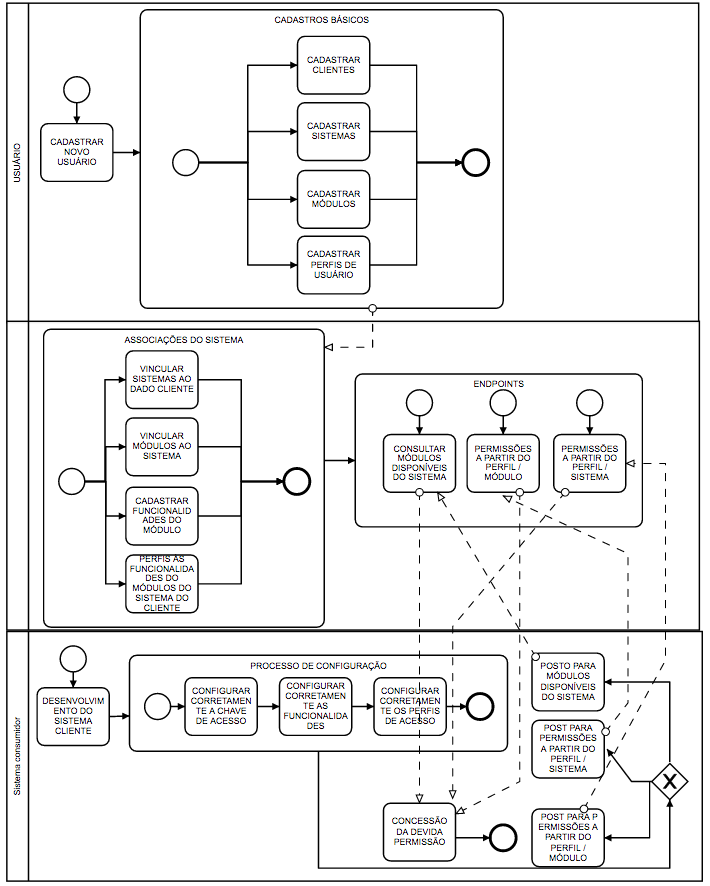
\includegraphics[width=1.3\linewidth]{img/diagrama_bpmn}
	}
	\label{fig:diagramaBpmn}
	\caption{Diagrama do processo(BPMN) do software em questão}
\end{figure}


\subsection{O que há de novo ?} %Sob o ponto de vista tecnológico


Seguindo a norma de padranização de código, com o software proposto é possível unificar o módulo de permissões de acesso e tratá-lo como um serviço, tornando possível eliminá-lo de qualquer software que faça uso do mesmo.